\documentclass[10pt,letterpaper,fleqn]{article}

\usepackage[utf8]{inputenc}
\usepackage[spanish,es-nodecimaldot]{babel}
\usepackage{amsmath}
\usepackage{amssymb}
\usepackage{multicol}
\usepackage{graphicx}
\usepackage{cancel}
\usepackage{enumerate}
\usepackage{colortbl}
\usepackage[dvipsnames,table,xcdraw]{xcolor}
\usepackage[most]{tcolorbox}
\usepackage{ upgreek }
\usepackage{tabu}
\usepackage{pgfplots}
\pgfplotsset{width=10cm,compat=1.9}

\usepackage{mathtools}
\usepackage{tikz}
\usetikzlibrary{trees,positioning}

\newcommand{\tablaRXS}{
\centering
\begin{tabular}{clllclccccc}
\rowcolor[HTML]{343434} 
\multicolumn{11}{c}{\cellcolor[HTML]{343434}{\color[HTML]{FFFFFF} RXS}} \\ \cline{1-5} \cline{7-11} 
\rowcolor[HTML]{9B9B9B} 
\multicolumn{1}{|c|}{\cellcolor[HTML]{9B9B9B}A} & \multicolumn{1}{c|}{\cellcolor[HTML]{9B9B9B}B} & \multicolumn{1}{c|}{\cellcolor[HTML]{9B9B9B}B} & \multicolumn{1}{c|}{\cellcolor[HTML]{9B9B9B}C} & \multicolumn{1}{c|}{\cellcolor[HTML]{9B9B9B}D} & \multicolumn{1}{l|}{\cellcolor[HTML]{FFFFFF}} & \multicolumn{1}{c|}{\cellcolor[HTML]{9B9B9B}A} & \multicolumn{1}{c|}{\cellcolor[HTML]{9B9B9B}B} & \multicolumn{1}{c|}{\cellcolor[HTML]{9B9B9B}B} & \multicolumn{1}{c|}{\cellcolor[HTML]{9B9B9B}C} & \multicolumn{1}{c|}{\cellcolor[HTML]{9B9B9B}D} \\ \cline{1-5} \cline{7-11} 
\multicolumn{1}{|c|}{2} & \multicolumn{1}{c|}{m} & \multicolumn{1}{c|}{m} & \multicolumn{1}{c|}{0} & \multicolumn{1}{c|}{6} & \multicolumn{1}{l|}{\cellcolor[HTML]{FFFFFF}} & \multicolumn{1}{c|}{4} & \multicolumn{1}{c|}{o} & \multicolumn{1}{c|}{p} & \multicolumn{1}{c|}{6} & \multicolumn{1}{c|}{0} \\ \cline{1-5} \cline{7-11} 
\rowcolor[HTML]{9B9B9B} 
\multicolumn{1}{|c|}{\cellcolor[HTML]{9B9B9B}2} & \multicolumn{1}{c|}{\cellcolor[HTML]{9B9B9B}m} & \multicolumn{1}{c|}{\cellcolor[HTML]{9B9B9B}n} & \multicolumn{1}{c|}{\cellcolor[HTML]{9B9B9B}4} & \multicolumn{1}{c|}{\cellcolor[HTML]{9B9B9B}2} & \multicolumn{1}{l|}{\cellcolor[HTML]{FFFFFF}} & \multicolumn{1}{c|}{\cellcolor[HTML]{9B9B9B}4} & \multicolumn{1}{c|}{\cellcolor[HTML]{9B9B9B}o} & \multicolumn{1}{c|}{\cellcolor[HTML]{9B9B9B}n} & \multicolumn{1}{c|}{\cellcolor[HTML]{9B9B9B}4} & \multicolumn{1}{c|}{\cellcolor[HTML]{9B9B9B}0} \\ \cline{1-5} \cline{7-11} 
\multicolumn{1}{|c|}{2} & \multicolumn{1}{c|}{m} & \multicolumn{1}{c|}{n} & \multicolumn{1}{c|}{6} & \multicolumn{1}{c|}{6} & \multicolumn{1}{l|}{\cellcolor[HTML]{FFFFFF}} & \multicolumn{1}{c|}{6} & \multicolumn{1}{c|}{m} & \multicolumn{1}{c|}{m} & \multicolumn{1}{c|}{0} & \multicolumn{1}{c|}{6} \\ \cline{1-5} \cline{7-11} 
\rowcolor[HTML]{9B9B9B} 
\multicolumn{1}{|c|}{\cellcolor[HTML]{9B9B9B}2} & \multicolumn{1}{c|}{\cellcolor[HTML]{9B9B9B}m} & \multicolumn{1}{c|}{\cellcolor[HTML]{9B9B9B}p} & \multicolumn{1}{c|}{\cellcolor[HTML]{9B9B9B}6} & \multicolumn{1}{c|}{\cellcolor[HTML]{9B9B9B}0} & \multicolumn{1}{l|}{\cellcolor[HTML]{FFFFFF}} & \multicolumn{1}{c|}{\cellcolor[HTML]{9B9B9B}6} & \multicolumn{1}{c|}{\cellcolor[HTML]{9B9B9B}m} & \multicolumn{1}{c|}{\cellcolor[HTML]{9B9B9B}n} & \multicolumn{1}{c|}{\cellcolor[HTML]{9B9B9B}4} & \multicolumn{1}{c|}{\cellcolor[HTML]{9B9B9B}2} \\ \cline{1-5} \cline{7-11} 
\multicolumn{1}{|c|}{2} & \multicolumn{1}{c|}{m} & \multicolumn{1}{c|}{n} & \multicolumn{1}{c|}{4} & \multicolumn{1}{c|}{0} & \multicolumn{1}{l|}{\cellcolor[HTML]{FFFFFF}} & \multicolumn{1}{c|}{6} & \multicolumn{1}{c|}{m} & \multicolumn{1}{c|}{n} & \multicolumn{1}{c|}{6} & \multicolumn{1}{c|}{6} \\ \cline{1-5} \cline{7-11} 
\rowcolor[HTML]{9B9B9B} 
\multicolumn{1}{|c|}{\cellcolor[HTML]{9B9B9B}4} & \multicolumn{1}{c|}{\cellcolor[HTML]{9B9B9B}n} & \multicolumn{1}{c|}{\cellcolor[HTML]{9B9B9B}m} & \multicolumn{1}{c|}{\cellcolor[HTML]{9B9B9B}0} & \multicolumn{1}{c|}{\cellcolor[HTML]{9B9B9B}6} & \multicolumn{1}{l|}{\cellcolor[HTML]{FFFFFF}} & \multicolumn{1}{c|}{\cellcolor[HTML]{9B9B9B}6} & \multicolumn{1}{c|}{\cellcolor[HTML]{9B9B9B}m} & \multicolumn{1}{c|}{\cellcolor[HTML]{9B9B9B}p} & \multicolumn{1}{c|}{\cellcolor[HTML]{9B9B9B}6} & \multicolumn{1}{c|}{\cellcolor[HTML]{9B9B9B}0} \\ \cline{1-5} \cline{7-11} 
\multicolumn{1}{|l|}{4} & \multicolumn{1}{l|}{n} & \multicolumn{1}{l|}{n} & \multicolumn{1}{l|}{4} & \multicolumn{1}{c|}{2} & \multicolumn{1}{l|}{\cellcolor[HTML]{FFFFFF}} & \multicolumn{1}{c|}{6} & \multicolumn{1}{c|}{m} & \multicolumn{1}{c|}{n} & \multicolumn{1}{c|}{4} & \multicolumn{1}{c|}{0} \\ \cline{1-5} \cline{7-11} 
\rowcolor[HTML]{9B9B9B} 
\multicolumn{1}{|l|}{\cellcolor[HTML]{9B9B9B}4} & \multicolumn{1}{l|}{\cellcolor[HTML]{9B9B9B}n} & \multicolumn{1}{l|}{\cellcolor[HTML]{9B9B9B}n} & \multicolumn{1}{l|}{\cellcolor[HTML]{9B9B9B}6} & \multicolumn{1}{c|}{\cellcolor[HTML]{9B9B9B}6} & \multicolumn{1}{l|}{\cellcolor[HTML]{9B9B9B}} & \multicolumn{1}{c|}{\cellcolor[HTML]{9B9B9B}8} & \multicolumn{1}{c|}{\cellcolor[HTML]{9B9B9B}z} & \multicolumn{1}{c|}{\cellcolor[HTML]{9B9B9B}m} & \multicolumn{1}{c|}{\cellcolor[HTML]{9B9B9B}0} & \multicolumn{1}{c|}{\cellcolor[HTML]{9B9B9B}6} \\ \cline{1-5} \cline{7-11} 
\multicolumn{1}{|l|}{4} & \multicolumn{1}{l|}{n} & \multicolumn{1}{l|}{p} & \multicolumn{1}{l|}{6} & \multicolumn{1}{c|}{0} & \multicolumn{1}{l|}{\cellcolor[HTML]{FFFFFF}} & \multicolumn{1}{c|}{8} & \multicolumn{1}{c|}{z} & \multicolumn{1}{c|}{n} & \multicolumn{1}{c|}{4} & \multicolumn{1}{c|}{2} \\ \cline{1-5} \cline{7-11} 
\rowcolor[HTML]{9B9B9B} 
\multicolumn{1}{|l|}{\cellcolor[HTML]{9B9B9B}4} & \multicolumn{1}{l|}{\cellcolor[HTML]{9B9B9B}n} & \multicolumn{1}{l|}{\cellcolor[HTML]{9B9B9B}n} & \multicolumn{1}{l|}{\cellcolor[HTML]{9B9B9B}4} & \multicolumn{1}{c|}{\cellcolor[HTML]{9B9B9B}0} & \multicolumn{1}{l|}{\cellcolor[HTML]{FFFFFF}} & \multicolumn{1}{c|}{\cellcolor[HTML]{9B9B9B}8} & \multicolumn{1}{c|}{\cellcolor[HTML]{9B9B9B}z} & \multicolumn{1}{c|}{\cellcolor[HTML]{9B9B9B}n} & \multicolumn{1}{c|}{\cellcolor[HTML]{9B9B9B}6} & \multicolumn{1}{c|}{\cellcolor[HTML]{9B9B9B}6} \\ \cline{1-5} \cline{7-11} 
\multicolumn{1}{|l|}{4} & \multicolumn{1}{l|}{o} & \multicolumn{1}{l|}{m} & \multicolumn{1}{l|}{0} & \multicolumn{1}{c|}{6} & \multicolumn{1}{l|}{\cellcolor[HTML]{FFFFFF}} & \multicolumn{1}{c|}{8} & \multicolumn{1}{c|}{z} & \multicolumn{1}{c|}{p} & \multicolumn{1}{c|}{6} & \multicolumn{1}{c|}{0} \\ \cline{1-5} \cline{7-11} 
\rowcolor[HTML]{9B9B9B} 
\multicolumn{1}{|l|}{\cellcolor[HTML]{9B9B9B}4} & \multicolumn{1}{l|}{\cellcolor[HTML]{9B9B9B}o} & \multicolumn{1}{l|}{\cellcolor[HTML]{9B9B9B}n} & \multicolumn{1}{l|}{\cellcolor[HTML]{9B9B9B}4} & \multicolumn{1}{c|}{\cellcolor[HTML]{9B9B9B}2} & \multicolumn{1}{l|}{\cellcolor[HTML]{FFFFFF}} & \multicolumn{1}{c|}{\cellcolor[HTML]{9B9B9B}8} & \multicolumn{1}{c|}{\cellcolor[HTML]{9B9B9B}z} & \multicolumn{1}{c|}{\cellcolor[HTML]{9B9B9B}n} & \multicolumn{1}{c|}{\cellcolor[HTML]{9B9B9B}4} & \multicolumn{1}{c|}{\cellcolor[HTML]{9B9B9B}0} \\ \cline{1-5} \cline{7-11} 
\multicolumn{1}{|l|}{4} & \multicolumn{1}{l|}{o} & \multicolumn{1}{l|}{n} & \multicolumn{1}{l|}{6} & \multicolumn{1}{c|}{6} & \cellcolor[HTML]{FFFFFF} &  &  &  &  &  \\ \cline{1-5}
\end{tabular}
}
\newcommand{\tablaRBS}{
\centering
\begin{tabular}{|c|c|c|c|}
\hline
\rowcolor[HTML]{000000} 
\multicolumn{4}{|c|}{\cellcolor[HTML]{000000}{\color[HTML]{FFFFFF} R$\bowtie$S}} \\ \hline
\rowcolor[HTML]{9B9B9B} 
A & B & C & D \\ \hline
2 & m & 0 & 6 \\ \hline
\rowcolor[HTML]{9B9B9B} 
4 & n & 4 & 2 \\ \hline
4 & n & 6 & 6 \\ \hline
\rowcolor[HTML]{9B9B9B} 
4 & n & 4 & 0 \\ \hline
6 & m & 0 & 6 \\ \hline
\end{tabular}
}
\newcommand{\tablaRLS}{
\centering
\begin{tabular}{|c|c|c|c|}
\hline
\rowcolor[HTML]{000000} 
\multicolumn{4}{|c|}{\cellcolor[HTML]{000000}{\color[HTML]{FFFFFF} R$\leftouterjoin$S}} \\ \hline
\rowcolor[HTML]{9B9B9B} 
A & B & C & D \\ \hline
2 & m & 0 & 6 \\ \hline
\rowcolor[HTML]{9B9B9B} 
4 & n & 4 & 2 \\ \hline
4 & n & 6 & 6 \\ \hline
\rowcolor[HTML]{9B9B9B} 
4 & n & 4 & 0 \\ \hline
4 & 0 & null & null \\ \hline
\rowcolor[HTML]{9B9B9B} 
6 & m & 0 & 6 \\ \hline
8 & z & null & null \\ \hline
\end{tabular}
}
\newcommand{\tablaRRS}{
\centering
\begin{tabular}{|c|c|c|c|}
\hline
\rowcolor[HTML]{000000} 
\multicolumn{4}{|c|}{\cellcolor[HTML]{000000}{\color[HTML]{FFFFFF} R$\rightouterjoin$S}} \\ \hline
\rowcolor[HTML]{9B9B9B} 
A & B & C & D \\ \hline
2 & m & 0 & 6 \\ \hline
\rowcolor[HTML]{9B9B9B} 
4 & n & 4 & 2 \\ \hline
4 & n & 6 & 6 \\ \hline
\rowcolor[HTML]{9B9B9B} 
4 & n & 4 & 0 \\ \hline
null & p & 6 & 0 \\ \hline
\rowcolor[HTML]{9B9B9B} 
6 & m & 0 & 6 \\ \hline
\end{tabular}
}
\newcommand{\tablaRS}{
\centering
\begin{tabular}{|c|c|c|c|}
\hline
\rowcolor[HTML]{000000} 
\multicolumn{4}{|c|}{\cellcolor[HTML]{000000}{\color[HTML]{FFFFFF} R$\bowtie_{A=D}$S}} \\ \hline
\rowcolor[HTML]{9B9B9B} 
A & B & C & D \\ \hline
6 & m & 0 & 6 \\ \hline
\end{tabular}
}
\newcommand{\tablaRCS}{
\centering
\begin{tabular}{|c|c|c|}
\hline
\rowcolor[HTML]{000000} 
\multicolumn{3}{|c|}{\cellcolor[HTML]{000000}{\color[HTML]{FFFFFF} $\rho_{\textbf{C}\xleftarrow{}\textbf{A}}$(R) $\bowtie$ S}} \\ \hline
\rowcolor[HTML]{9B9B9B} 
B & C & D \\ \hline
n & 4 & 2 \\ \hline
\rowcolor[HTML]{9B9B9B} 
n & 4 & 0 \\ \hline
\end{tabular}
}
\newcommand{\tablaRBBS}{
\centering
\begin{tabular}{|c|}
\hline
\rowcolor[HTML]{000000} 
{\color[HTML]{FFFFFF} $\pi$_{\:B}(R) - $\pi_{\:B}$ ($\sigma_{\: c < 3}$(S))} \\ \hline
\rowcolor[HTML]{9B9B9B} 
B \\ \hline
n \\ \hline
\rowcolor[HTML]{9B9B9B} 
o \\ \hline
z \\ \hline
\end{tabular}
}
\newcommand{\tablaRBBBS}{
\centering
\begin{tabular}{|c|}
\hline
\rowcolor[HTML]{000000} 
{\color[HTML]{FFFFFF} $\pi$_{\:A}(R) $\cap$ $\rho_{\:A \leftarrow D }$ ($\pi_{\:D}$(S))} \\ \hline
\rowcolor[HTML]{9B9B9B} 
A \\ \hline
2 \\ \hline
\rowcolor[HTML]{9B9B9B} 
6 \\ \hline
\end{tabular}
}
\newcommand{\tablaRBBBBS}{
\centering
\begin{tabular}{|c|c|c|}
\hline
\rowcolor[HTML]{000000} 
\multicolumn{3}{|c|}{\cellcolor[HTML]{000000}{\color[HTML]{FFFFFF}$\pi$_{\:D}(S) $\bowtie$ S}} \\ \hline
\rowcolor[HTML]{9B9B9B} 
B & C & D \\ \hline
m & 0 & 6 \\ \hline
\rowcolor[HTML]{9B9B9B} 
n & 4 & 2 \\ \hline
n & 6 & 6 \\ \hline
\rowcolor[HTML]{9B9B9B} 
p & 6 & 0 \\ \hline
n & 4 & 0 \\ \hline
\end{tabular}
}
\newcommand{\tablaRBBBBBS}{
\centering
\begin{tabular}{|c|c|}
\hline
\rowcolor[HTML]{000000} 
\multicolumn{2}{|c|}{\cellcolor[HTML]{000000}{\color[HTML]{FFFFFF} $\Upsilon$A;count(B) $\rightarrow$ t(R \fullouterjoin S)}} \\ \hline
\rowcolor[HTML]{9B9B9B} 
A & t \\ \hline
2 & 1 \\ \hline
\rowcolor[HTML]{9B9B9B} 
4 & 4 \\ \hline
6 & 1 \\ \hline
\rowcolor[HTML]{9B9B9B} 
8 & 1 \\ \hline
\end{tabular}
}
\usepackage[top=1in, bottom=1in, left=1in, right=1in]{geometry}
%\graphicspath{ {../../assets/img/logo.png} }
\def\ojoin{\setbox0=\hbox{$\bowtie$}%
  \rule[-.02ex]{.25em}{.4pt}\llap{\rule[\ht0]{.25em}{.4pt}}}
\def\leftouterjoin{\mathbin{\ojoin\mkern-5.8mu\bowtie}}
\def\rightouterjoin{\mathbin{\bowtie\mkern-5.8mu\ojoin}}
\def\fullouterjoin{\mathbin{\ojoin\mkern-5.8mu\bowtie\mkern-5.8mu\ojoin}}

\begin{document}
    \begin{titlepage}
        \centering
    
        {\scshape\LARGE Universidad Nacional Autónoma de México \par}
    
        \vspace{1cm}
        {\scshape\Large Facultad de ciencias\par}
        \vspace{1.5cm}
    
        \begin{center}
            \includegraphics[scale=.1]{../../../assets/img/logo.png}
        \end{center}
    
        \vspace{.8 cm}
    
        {\LARGE Tarea 3: \par}
        {\huge\bfseries Álgebra relacional \par}
    
        \vspace{0.5cm}
        %Nombres y números de cuenta%
        \large{\itshape{Angel Christian Pimentel Noriega}} \small{ - 316157995 } \\
        \large{\itshape{Mauricio Riva Palacio Orozco}} \small{ - 316666343 } \\
        \large{\itshape{Alex Gerardo Fernandez Aguilar }} \small{ - 314338097  } \\
        \large{\itshape{Martin Felipe Espinal Cruces}} \small{ - 316155362 } \\
        \vfill
        \vfill
        Trabajo presentado como parte del curso de
        \textbf{Fundamentos de Bases de Datos}
        impartido por el profesor \textbf{ Gerardo Avíles Rosas }. \par
        \vspace{0.1cm}
    \end{titlepage}
    \begin{enumerate}
        %1%
        \item \textbf{Cardinalidad de la consulta}\\
        Considera las siguientes relaciones:
        \begin{center}
            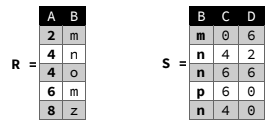
\includegraphics[scale=2]{psets/Tareas/Tarea03/Diagramas/1.png}
        \end{center}
        Para las siguientes expresiones de \textbf{álgebra relacional} completa la tabla con el conjunto de tuplas que cada una de ellas produce utilizando las relaciones \textbf{R} y  \textbf{S}
        \begin{center}
            %Tabla%
            \begin{tabular}{|l|l|}
            \hline
            \cellcolor{black}\textcolor{white}{Expresión} & \cellcolor{black}\textcolor{white}{Tuplas resultantes}\\
            \hline
            \cellcolor{gray}\textbf{R x S} & \cellcolor{gray}\\
            \hline 
            \textbf{R $\bowtie$ S} & \\
            \hline
            \cellcolor{gray}\textbf{R $\leftouterjoin$ S} & \cellcolor{gray}\\
            \hline
            \textbf{R $\rightouterjoin$ S} & \\
            \hline
            \cellcolor{gray}\textbf{R $\bowtie_{A=D}$ S} & \cellcolor{gray}\\
            \hline
            \textbf{$\rho_{\textbf{C}\xleftarrow{}\textbf{A}}$(R) $\bowtie$ S} & \\
            \hline
             \cellcolor{gray}\textbf{$\pi_{\:B}$(R) - $\pi_{\:B}$ ($\sigma_{\: c < 3}$(S))} &  \cellcolor{gray}\\
            \hline

             \textbf{$\pi_{\:A}$(R) $\cap$ $\rho_{\:A \leftarrow D }$ ($\pi_{\:D}$(S))} & \\
            \hline
            
            \cellcolor{gray}\textbf{$\pi_{\:D}$(S) $\bowtie$ S} &  \cellcolor{gray}\\
            \hline
            
            \textbf{$\Upsilon$_{\:A;count(B) $\rightarrow$ t}(R \fullouterjoin S)} & \\
            \hline
            
            \end{tabular}
        \end{center}
        %Aqui quiero que quede la tabla
        \begin{center}
            \tablaRXS
        \end{center}
        \begin{center}
            \tablaRBS
        \end{center}
        \begin{center}
            \tablaRLS
        \end{center}
        \begin{center}
            \tablaRRS
        \end{center}
        \begin{center}
            \tablaRS
        \end{center}
        \begin{center}
            \tablaRCS
        \end{center}
        \begin{center}
            \tablaRBBS
        \end{center}
         \begin{center}
            \tablaRBBBS
        \end{center}
        \begin{center}
            \tablaRBBBBS
        \end{center}
        \begin{center}
            \tablaRBBBBBS
        \end{center}
        
        %2%
        \item \textbf{Banco del sur}
        Supón que tienes el siguiente \textbf{esquema de una base de datos} para una institución bancaria:
        \begin{center}
            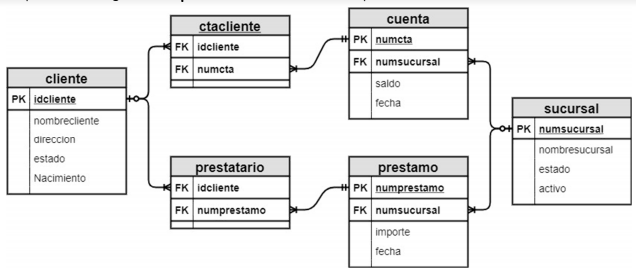
\includegraphics[scale=3]{psets/Tareas/Tarea03/Diagramas/2.png}
        \end{center}
        Escribe una \textbf{expresión de álgebra relacional} para responder las siguientes consultas. Deberás comprobar cada una ellas en \textbf{Relax} y agregar en cada inciso una captura de pantalla con el resultado obtenido:
        \begin{enumerate}[a]
            %2.a%
            \item Encontrar la información de todas las cuentas otorgadas en la sucursal \textbf{BONAMPAK} de \textbf{2013} a \textbf{2014}.
            \begin{enumerate}[1]
                \item \textbar \quad r = $\pi$ numsucursal ($\sigma$ nombresucursal = 'BONAMPAK' (sucursal))
                \item \textbar \quad s = cuenta $\bowtie$ r 
                \item \textbar \quad t = $\sigma$ fecha $\geq$ date('2013-01-01') s
                \item \textbar \quad u = $\sigma$ fecha $<$ date('2015-01-01') s 
                \item \textbar \quad t $\cap$ u 
            \end{enumerate}
            %2.b%
            \item Obtener toda la información de los clientes que viven en \textbf{DURANGO}, que hayan nacido después del 25 de \textbf{mayo de 1975} y que tengan algún préstamo. Mostrar la información \textbf{ordenada} por el nombre del cliente.
            \begin{enumerate}[1]
                \item \textbar \quad r = $\sigma$ estado = 'DURANGO' (cliente)
                \item \textbar \quad s = $\sigma$ nacimiento $>$ date('1975-05-25') r 
                \item \textbar \quad t = s $\bowtie$ prestatario
                \item \textbar \quad u = $\tau$ nombrecliente t 
                \item \textbar \quad $\pi$ nombrecliente, direccion, estado, nacimiento (u)
            \end{enumerate}
            %2.c%
            \item Toda la información de los clientes del banco que tiene una cuenta, un préstamo o ambas y que no vivan en \textbf{CHIAPAS}.
            \begin{enumerate}[1]
                \item \textbar \quad r = $\sigma$ estado $\neq$ 'CHIAPAS' (cliente)
                \item \textbar \quad s = r $\bowtie$ ctacliente
                \item \textbar \quad t = r $\bowtie$ prestatario
                \item \textbar \quad s $\cup$ t
            \end{enumerate}
            %2.d%
            \item Relación de los clientes que \textbf{tienen una cuenta} con un saldo mayor que $\$$ \textbf{75,000.00} y menor que $\$$\textbf{100,000.00}, pero \textbf{no tienen ningún préstamo} en el banco. Mostrar el \textbf{idcliente, nombre del cliente, número de préstamo e importe}.
            \begin{enumerate}[1]
                \item \textbar \quad r = $\sigma$ saldo $>$ 75000 cuenta
                \item \textbar \quad s = $\sigma$ saldo $<$ 100000 cuenta
                \item \textbar \quad t = r $\cap$ s
                \item \textbar \quad u = t $\bowtie$ ctacliente
                \item \textbar \quad v = $\pi$ idcliente, nombrecliente, direccion, estado, nacimiento (u $\bowtie$ cliente)
                \item \textbar \quad w = $\pi$ idcliente, nombrecliente, direccion, estado, nacimiento (prestatario $\bowtie$ v)
                \item \textbar \quad v - w
            \end{enumerate}
            %2.e%
            \item Todos los clientes que \textbf{tienen un préstamo} y una cuenta, que hayan nacido en \textbf{GUANAJUATO} o \textbf{ZACATECAS}.
            \begin{enumerate}[1]
                \item \textbar \quad r = $\sigma$ estado = 'GUANAJUATO' (cliente)
                \item \textbar \quad s = $\sigma$ estado = 'ZACATECAS' (cliente)
                \item \textbar \quad p = ctacliente - prestatario
                \item \textbar \quad q = prestatario -ctacliente
                \item \textbar \quad (s $\bowtie$ p)  prestatario
                \item \textbar \quad (s $\bowtie$ p) $\cup$ (r $\bowtie$ q)
            \end{enumerate}
            %2.f%
            \item Información de los clientes que hayan nacido en \textbf{OAXACA} que no tienen crédito en sucursales de \textbf{OAXACA}.
            \begin{enumerate}[1]
                \item \textbar \quad r = $\sigma$ estado = 'OAXACA' (cliente)
                \item \textbar \quad s = $\sigma$ estado = 'OAXACA' (sucursal)
                \item \textbar \quad u = sucursal - s
                \item \textbar \quad t = r $\bowtie$ prestatario
                \item \textbar \quad u $\bowtie$ t
            \end{enumerate}
            Esta consulta no devolvió resultados debido a que la sucursal que se le asigna al usuario sea la que esta mas cerca de su casa, además que es muy poco probable ir a otro estado al banco.
            %2.g%
            \item Nombre de todos los clientes que tienen \textbf{una cuenta y el saldo} del mismo. El saldo no debe ser mayor de $\$$65,500, la cuenta se debió entregar durante el mes de \textbf{junio de 2013}.
            \begin{enumerate}[1]
                \item \textbar \quad r = $\sigma$ saldo $<$ 65500 $\wedge$ fecha $\geq$ date('2013-06-01') $\wedge$ fecha $\leq$ date('2013-06-30') (cuenta)
                \item \textbar \quad s = r $\bowtie$ ctacliente
                \item \textbar \quad s $\bowtie$ cliente
            \end{enumerate}
            %2.h%
            \item Toda la información de las sucursales con clientes que tengan un préstamo otorgado en el banco en alguna de las sucursales de \textbf{CAMPECHE} y que no viven en \textbf{CAMPECHE}.
            \begin{enumerate}[1]
                \item \textbar \quad r = $\sigma$ estado = 'CAMPECHE' (sucursal)
                \item \textbar \quad v = $\sigma$ estado $\neq$ 'CAMPECHE' (cliente)
                \item \textbar \quad s = r $\bowtie$ prestamo
                \item \textbar \quad t = v $\bowtie$ prestatario
                \item \textbar \quad s $\bowtie$ t
            \end{enumerate}
            Esta consulta no devolvió resultados debido a que es muy sospechoso que una persona vaya a otro estado en donde no vive para hacer un préstamo, el banco tratara de que todas la operaciones necesarias se puedan hacer en la sucursal mas cercana de la ubicación del usuario.
            %2.i%
            \item Toda la información de los clientes que tienen solo alguna cuenta entregada en \textbf{2014} y aquellos que tienen solo algún préstamo entregado durante \textbf{2015} el banco.
            \begin{enumerate}[1]
                \item \textbar \quad r = $\sigma$ fecha $\geq$ date('2014-01-01') $\land$ fecha $\leq$ date('2014-12-31') (cuenta)
                \item \textbar \quad r = $\sigma$ fecha $\geq$ date('2015-01-01') $\land$ fecha $\leq$ date('2015-12-31') (prestamo)
                \item \textbar \quad p = ctacliente - prestatario
                \item \textbar \quad q = prestatario -ctacliente 
                \item \textbar \quad (s $\bowtie$ p) $\cup$ (r $\bowtie$ q)
            \end{enumerate}
            %2.j%
            \item Una lista que muestre el estado, el nombre de sucursal y total de clientes que se tienen, considerando que los clientes deben tener un préstamo con saldo mayor a $\$$\textbf{60,000.00}, entregado de \textbf{2013} a \textbf{2015}.
            \begin{enumerate}[1]
                \item \textbar \quad r = $\sigma$ fecha $\geq$ date('2013-01-01') $\land$ fecha $\leq$ date('2015-12-31') (prestamo)
                \item \textbar \quad s = $\sigma$ importe $\leq$ 60000.00 (prestamo)
                \item \textbar \quad s = $\gamma$ COUNT(*) $\xrightarrow[]{}$ total (r $\bowtie$ s)
                \item \textbar \quad $\pi$ estado,nombresucursal,total (p $\bowtie$ sucursal)
            \end{enumerate}
            %2.k%
            \item Información de los clientes con saldo entre $\$$\textbf{15,000.00} y $\$$\textbf{30,000.00} que no han solicitado préstamos
            \begin{enumerate}[1]
                \item \textbar \quad r = $\sigma$ saldo $\geq$ 15000 $\land$ saldo $\leq$ 300000 (cuenta)
                \item \textbar \quad s = ctacliente - prestatario
                \item \textbar \quad cliente $\bowtie$ s $\bowtie$ r
            \end{enumerate}
            %2.l%
            \item Una lista con el \textbf{saldo promedio, mayor saldo, menor saldo, y total de cuenta}s, por estado y sucursal. El saldo promedio debe ser mayor que $\$$\textbf{85,000.00}
            \begin{enumerate}[1]
                \item \textbar \quad r = $\gamma$ estado;AVG(saldo) $\xrightarrow[]{}$ saldoProm (cuenta $\bowtie$ sucursal)
                \item \textbar \quad s = $\gamma$ estado;MIN(saldo) $\xrightarrow[]{}$ saldoMin (cuenta $\bowtie$ sucursal)
                \item \textbar \quad p = $\gamma$ estado;MAX(saldo) $\xrightarrow[]{}$ saldoMax (cuenta $\bowtie$ sucursal)
                \item \textbar \quad q = $\gamma$ estado;COUNT(*) $\xrightarrow[]{}$ total (cuenta $\bowtie$ sucursal)
                \item \textbar \quad t = $\sigma$ saldoProm $\xrightarrow[]{}$ 85000.00 (r))
                \item \textbar \quad u = t $\bowtie$ s $\bowtie$ p $\bowtie$ q
                \item \textbar \quad a = $\pi$ saldoProm,saldoMax,saldoMin,total (u)
                \item \textbar \quad c = $\gamma$ numsucursal;AVG(saldo) $\xrightarrow[]{}$ saldoProm (cuenta $\bowtie$ sucursal)
                \item \textbar \quad d = $\gamma$ numsucursal;MIN(saldo) $\xrightarrow[]{}$ saldoMin (cuenta $\bowtie$ sucursal)
                \item \textbar \quad e = $\gamma$ numsucursal;MAX(saldo) $\xrightarrow[]{}$ saldoMax (cuenta $\bowtie$ sucursal)
                \item \textbar \quad f = $\gamma$ numsucursal;COUNT(*) $\xrightarrow[]{}$ total (cuenta $\bowtie$ sucursal)
                \item \textbar \quad g = $\sigma$ saldoProm $\xrightarrow[]{}$ 85000.00 (r))
                \item \textbar \quad b = g $\bowtie$ d $\bowtie$ e $\bowtie$ f
                \item \textbar \quad a $\cup$ b
            \end{enumerate}
            %2.m%
            \item El estado que ha otorgado la \textbf{mayor cantidad de préstamos}, cuyo importe esté entre $\$$ \textbf{100,000.00} y $\$$\textbf{120,000.00}. Se debe mostrar también el total de préstamos.
            \begin{enumerate}[1]
                \item \textbar \quad r = $\gamma$ estado;COUNT(numprestamo) $\xrightarrow[]{}$ totalPrestamos (prestamo $\bowtie$ sucursal)
                \item \textbar \quad s = $\gamma$ MAX(saldo) $\xrightarrow[]{}$ saldoMax (r)
                \item \textbar \quad $\sigma$ (importe $\geq$ 100000.00 $\land$ importe $\leq$ 120000.00) prestamo $\bowtie$ sucursal $\bowtie$ s
            \end{enumerate}
            %2.n%
            \item El \textbf{id, nombre del cliente, sucursal y saldo} de aquel cliente que tenga el mayor saldo de todas las cuentas del banco.
            \begin{enumerate}[1]
                \item \textbar \quad r = $\gamma$ MAX(numprestamo) (saldo) $\xrightarrow[]{}$ Saldo (cuenta)
                \item \textbar \quad t = r $\bowtie$ ctacliente $\bowtie$ cliente $\bowtie$ prestatario $\bowtie$ prestamo
                \item \textbar \quad $\pi$ idcliente,nombrecliente,numsucursal,saldo (t $\bowtie$ r)
            \end{enumerate}
            %2.o%
            \item El \textbf{nombre de la sucursal y el saldo promedio}, de aquella que tiene el menor saldo promedio de todas las sucursales del banco.
            \begin{enumerate}[1]
                \item \textbar \quad r = $\gamma$ numsucursal;AVG(saldo) $\xrightarrow[]{}$ saldoProm (cuenta)
                \item \textbar \quad s = $\gamma$ MIN(saldoProm) $\xrightarrow[]{}$ min r
                \item \textbar \quad t = s $\bowtie$ sucursal
                \item \textbar \quad $\pi$ nombresucursal,saldoProm (t $\bowtie$ r)
            \end{enumerate}
        \end{enumerate}
        \textbf{Operaciones de mantenimiento de datos: borrado, inserción y actualización}
        \begin{enumerate}[a]
            %a%
            \item Borrar toda la información de la clienta \textbf{SUSANA BLANCO AGUILAR}.
            \begin{center}
            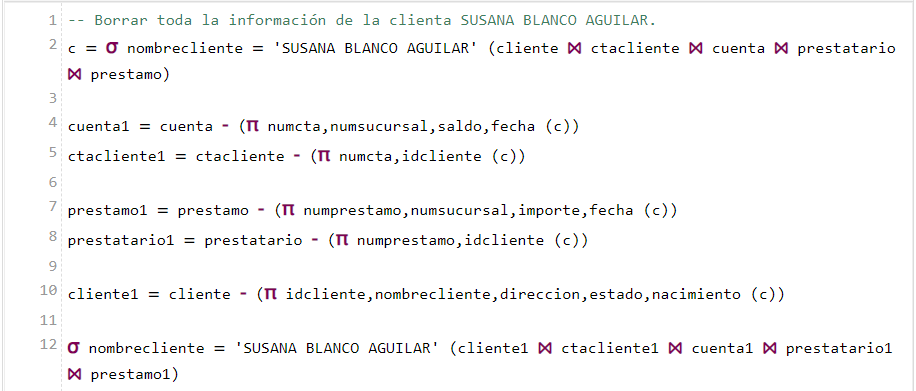
\includegraphics[scale=0.7]{psets/Tareas/Tarea03/Diagramas/2_2a.png}
            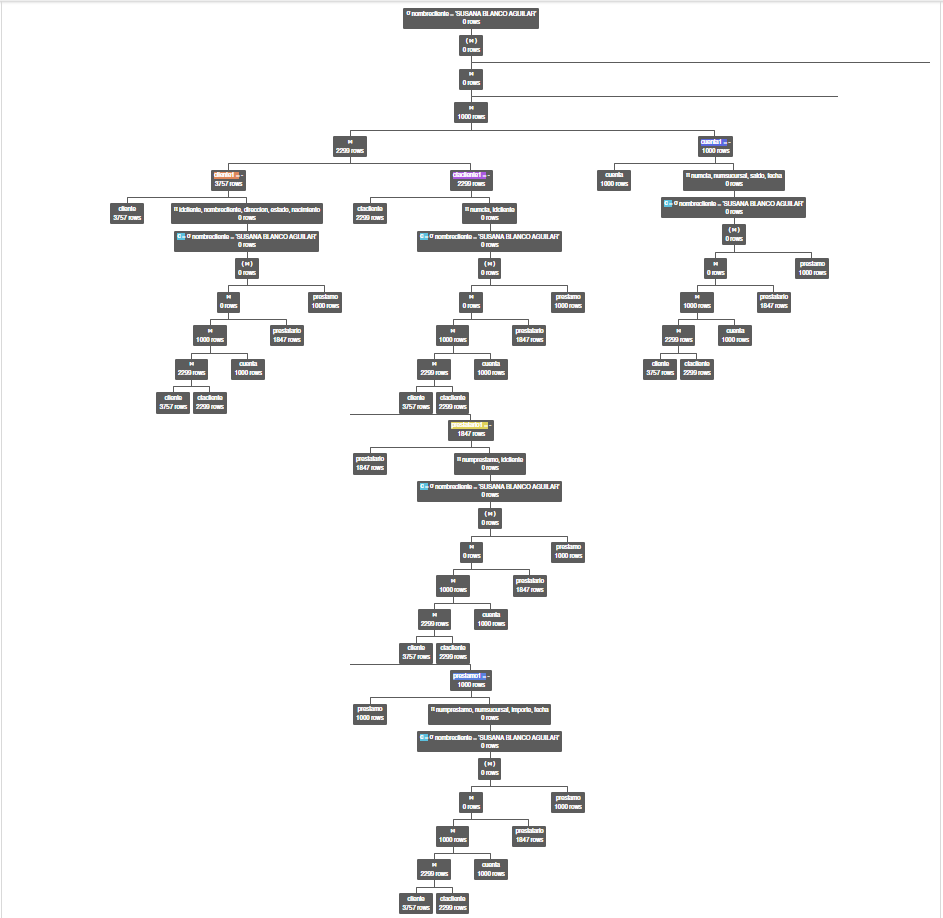
\includegraphics[scale=0.7]{psets/Tareas/Tarea03/Diagramas/2_2a0.png}
            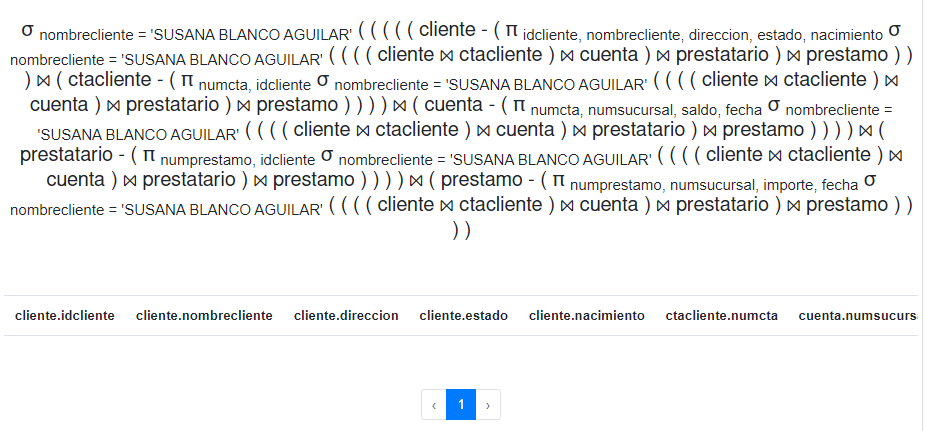
\includegraphics[scale=0.7]{psets/Tareas/Tarea03/Diagramas/2_2a1.png}
            \end{center}
            %b%
            \item Borrar todas las cuentas de la sucursal \textbf{UXMAL}.
            \begin{center}
            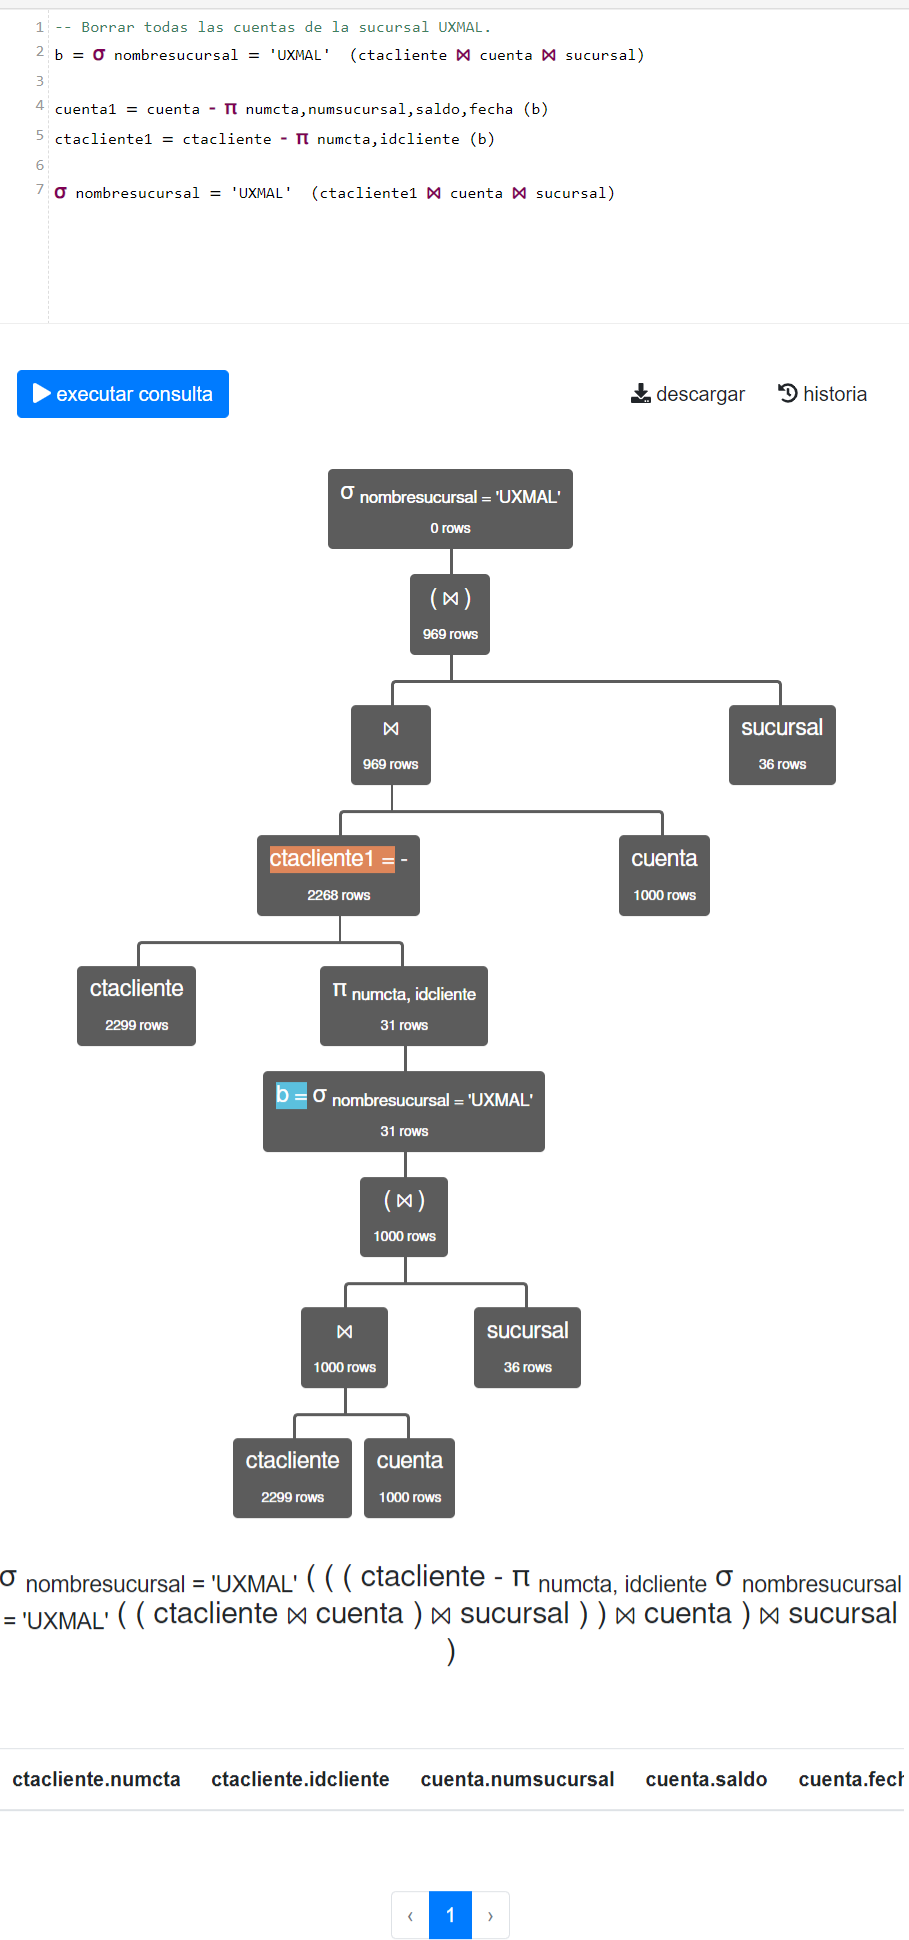
\includegraphics[scale=0.45]{psets/Tareas/Tarea03/Diagramas/2_2b.png}
            \end{center}
            %c%
            \item Borrar la información de las cuentas otorgadas durante \textbf{2013}.
            \begin{center}
            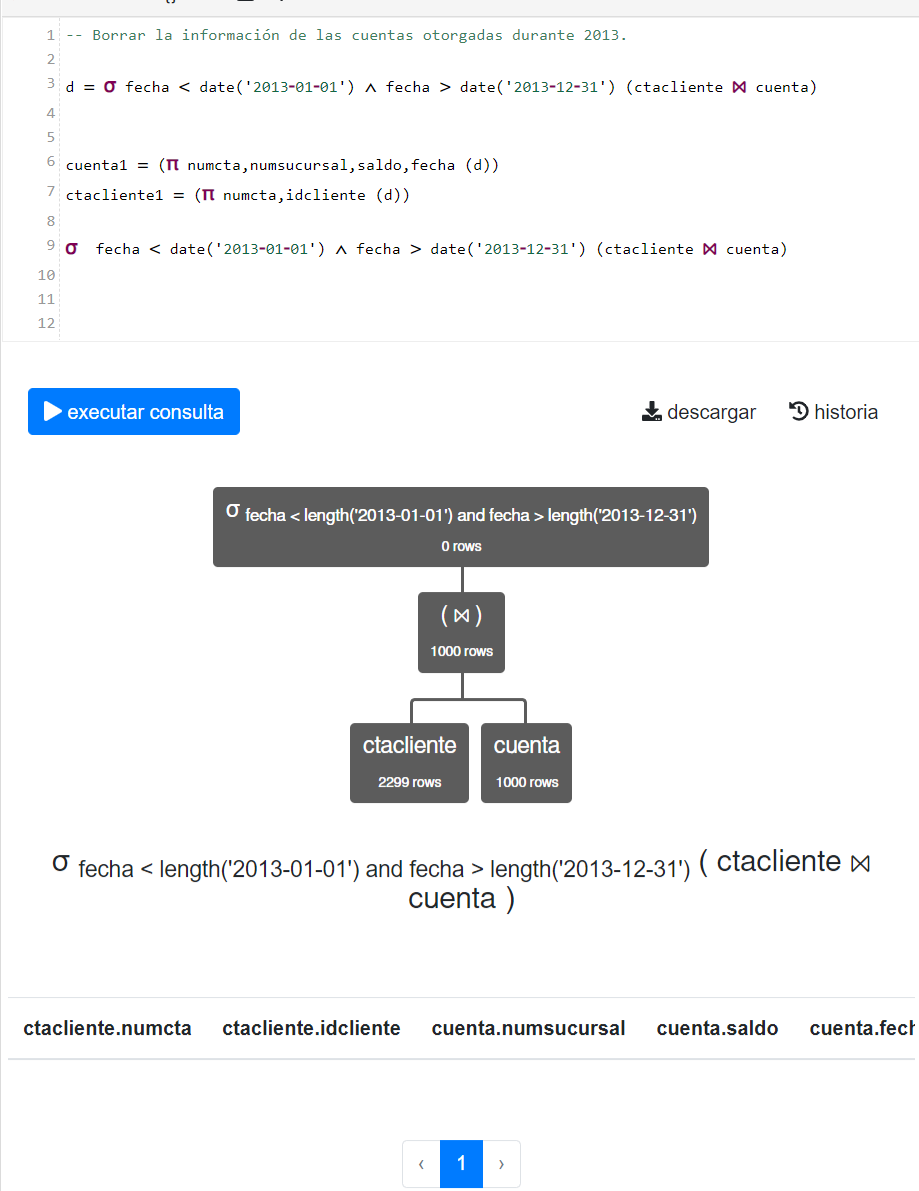
\includegraphics[scale=0.6]{psets/Tareas/Tarea03/Diagramas/2_2c.png}
            \end{center}
            %d %
            \item Otorgar el préstamo \textbf{P-05293} a la clienta \textbf{HÉCTOR NAVARRO LEÓN} con importe de $\$$\textbf{25,000}. El préstamo se otorgará en la misma sucursal donde tiene dada de alta su cuenta.
            \begin{center}
            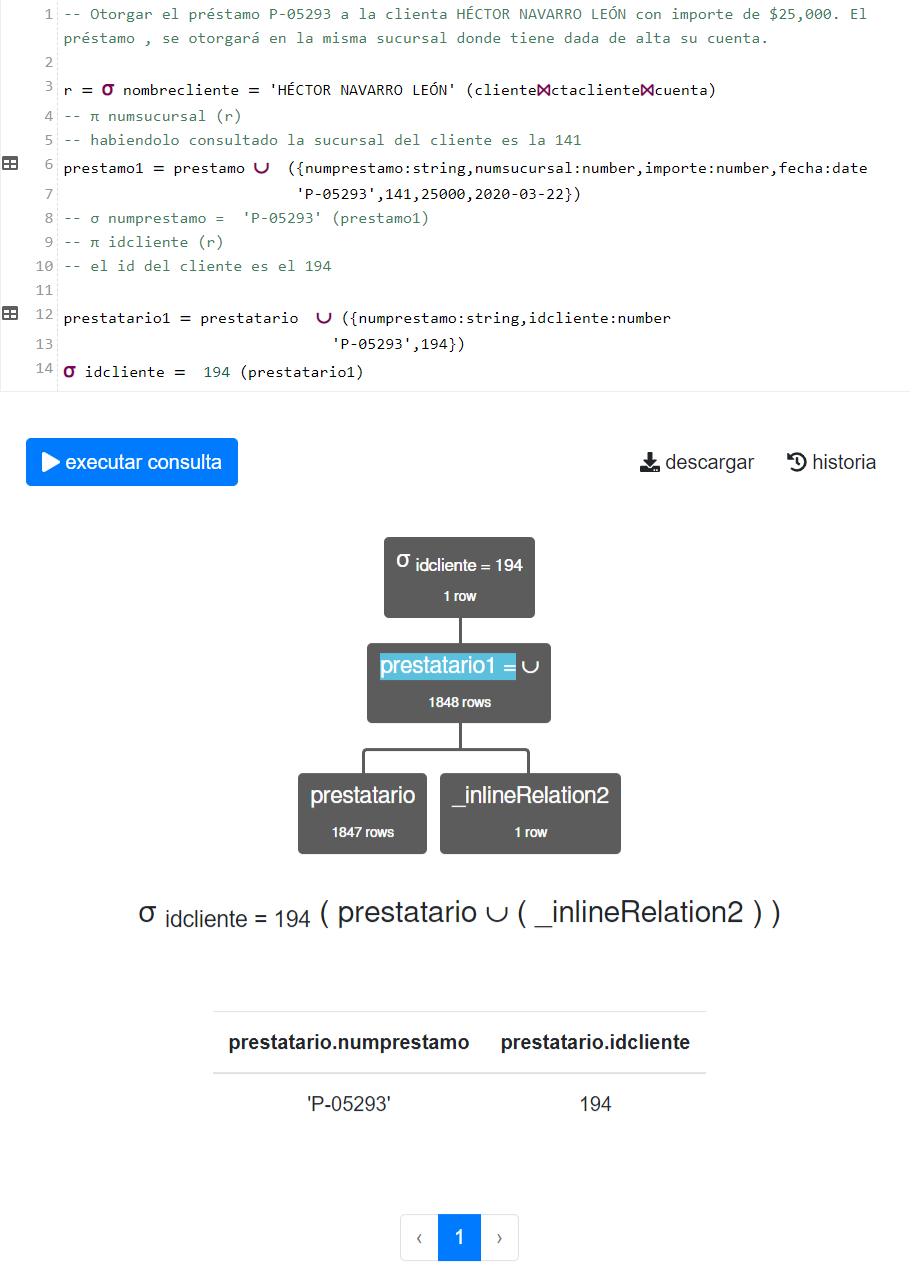
\includegraphics[scale=0.5]{psets/Tareas/Tarea03/Diagramas/2_2d.png}
            \end{center}
            %e%
            \item Ofrecer un nuevo préstamo con $\$$\textbf{30,000.00} a todos los clientes que tienen cuenta con saldo mayor de $\$$\textbf{80,000.00} en la sucursal \textbf{PROGRESO}, el número de préstamo será el de la nueva cuenta. Si el saldo es menor o igual a $\$$\textbf{80,000.00}, se les otorgará un préstamo de $\$$\textbf{15,000.00}.\\
            \begin{center}
            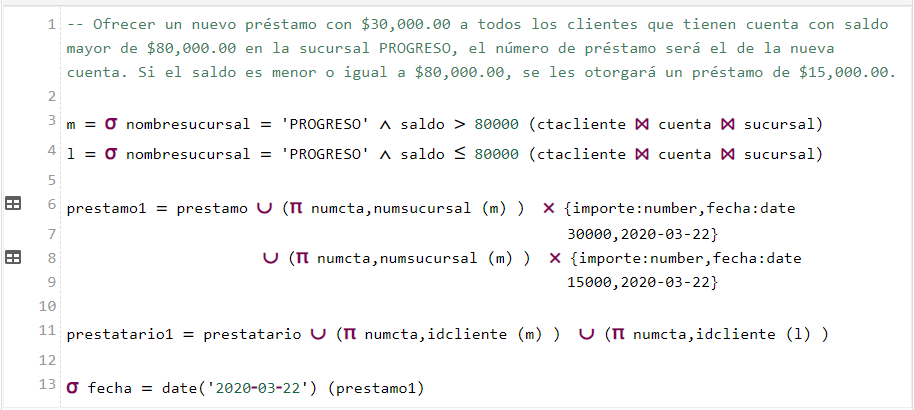
\includegraphics[scale=0.8]{psets/Tareas/Tarea03/Diagramas/2_2e.png}
            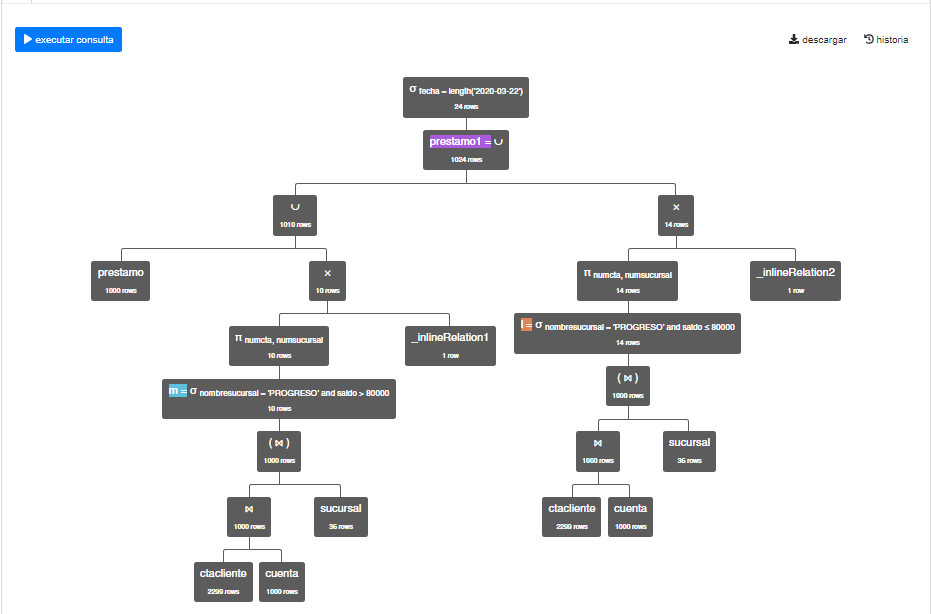
\includegraphics[scale=0.8]{psets/Tareas/Tarea03/Diagramas/2_2e0.png}
            \end{center}
            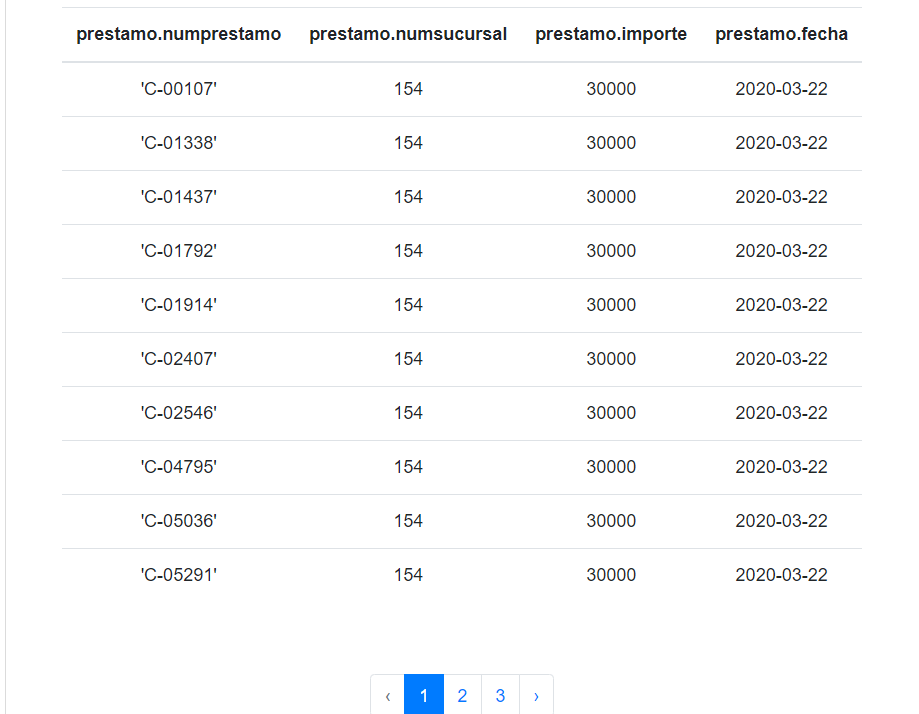
\includegraphics[scale=0.25]{psets/Tareas/Tarea03/Diagramas/2_2e1.png}
            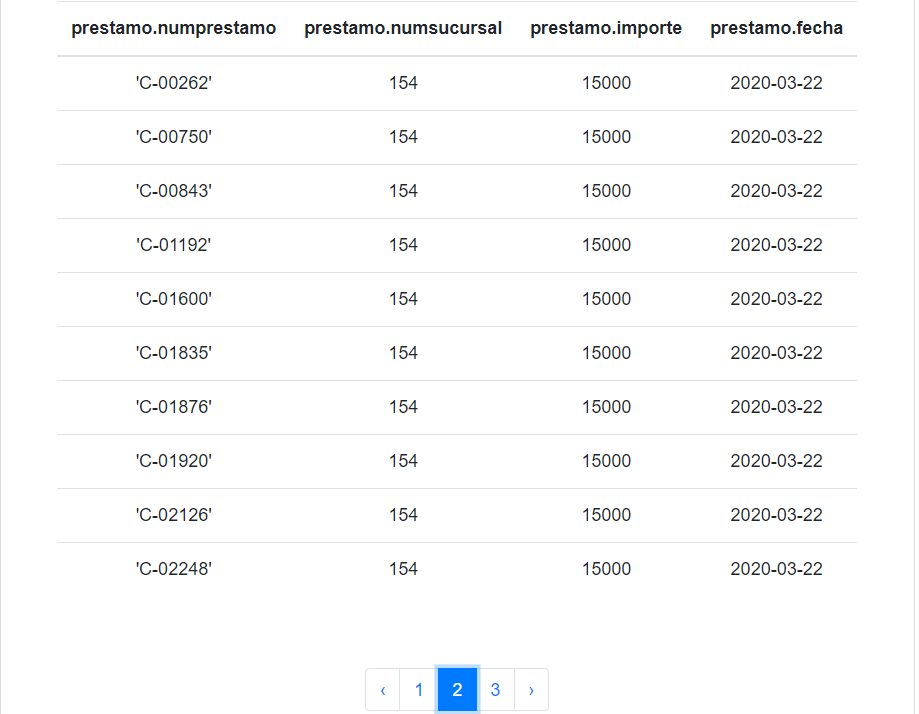
\includegraphics[scale=0.25]{psets/Tareas/Tarea03/Diagramas/2_2e2.png}
            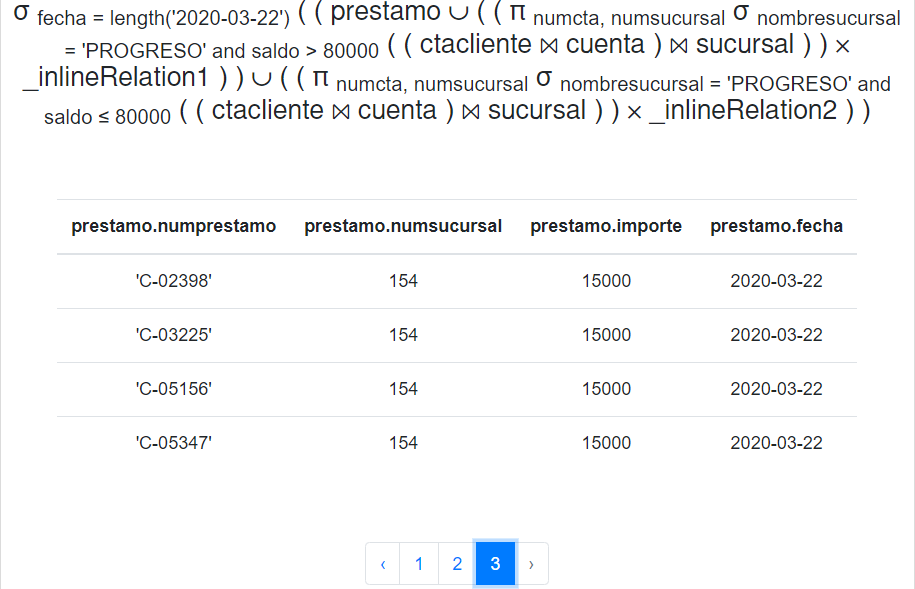
\includegraphics[scale=0.25]{psets/Tareas/Tarea03/Diagramas/2_2e3.png}
             
            %f%
            \item Disminuir el importe del préstamo de \textbf{DANIEL LOZANO GUERRERO} en un 17$\%$.
            \begin{center}
            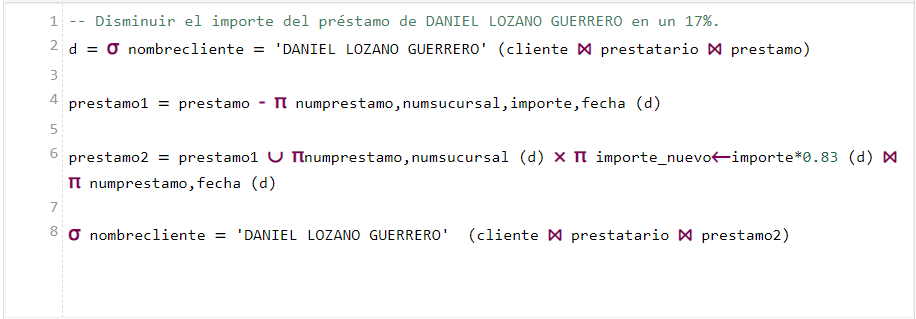
\includegraphics[scale=0.8]{psets/Tareas/Tarea03/Diagramas/2_2f0.png}
            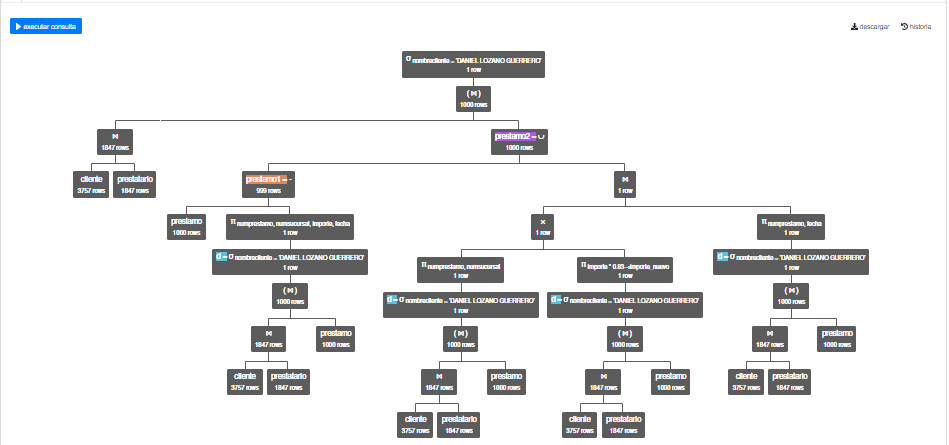
\includegraphics[scale=0.8]{psets/Tareas/Tarea03/Diagramas/2_2f1.png}
            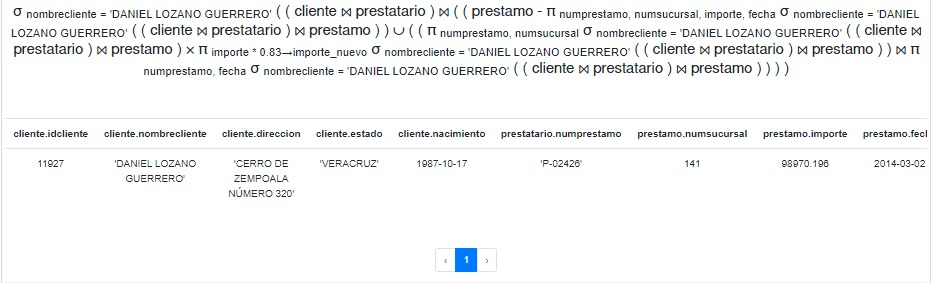
\includegraphics[scale=0.8]{psets/Tareas/Tarea03/Diagramas/2_2f2.png}
            \end{center}
            %g%
            \item Disminuir todos los saldos de la sucursal \textbf{CHUBURNA} en un \textbf{6}$\%$.
            \begin{center}
            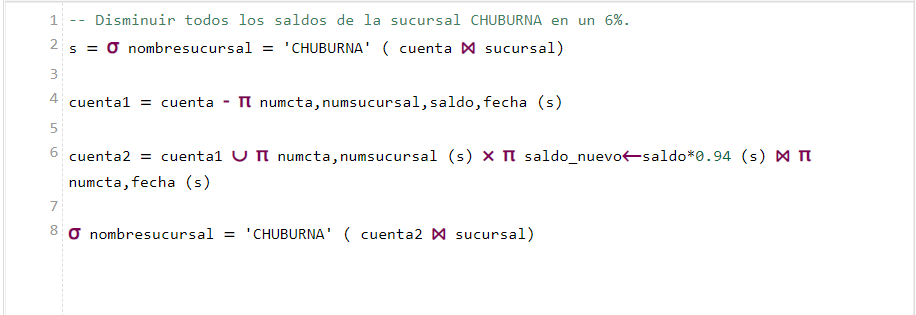
\includegraphics[scale=0.8]{psets/Tareas/Tarea03/Diagramas/2_2g0.png}
            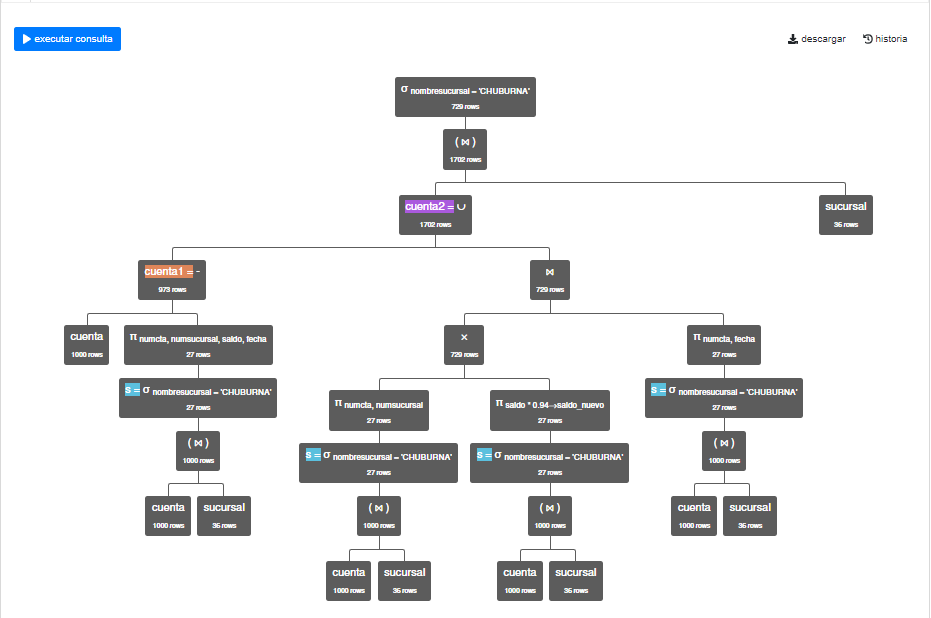
\includegraphics[scale=0.8]{psets/Tareas/Tarea03/Diagramas/2_2g1.png}
            \end{center}
            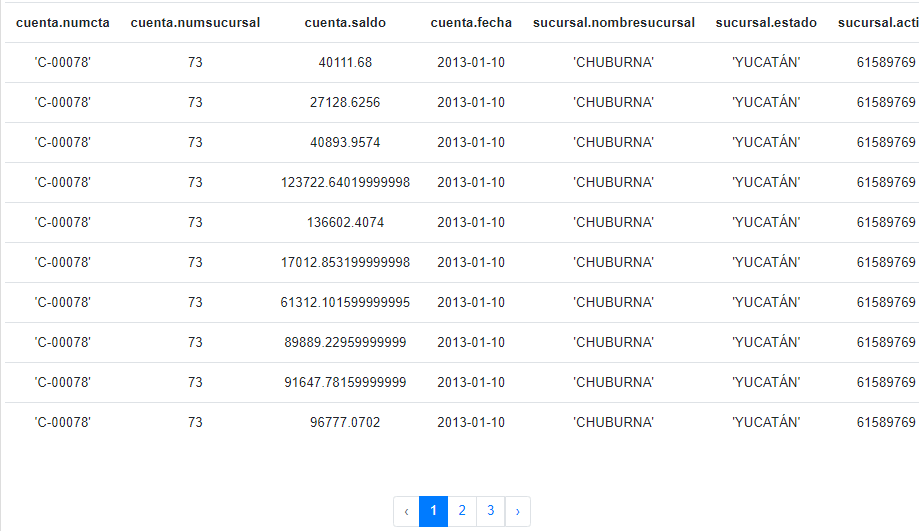
\includegraphics[scale=0.4]{psets/Tareas/Tarea03/Diagramas/2_2g2.png}    
            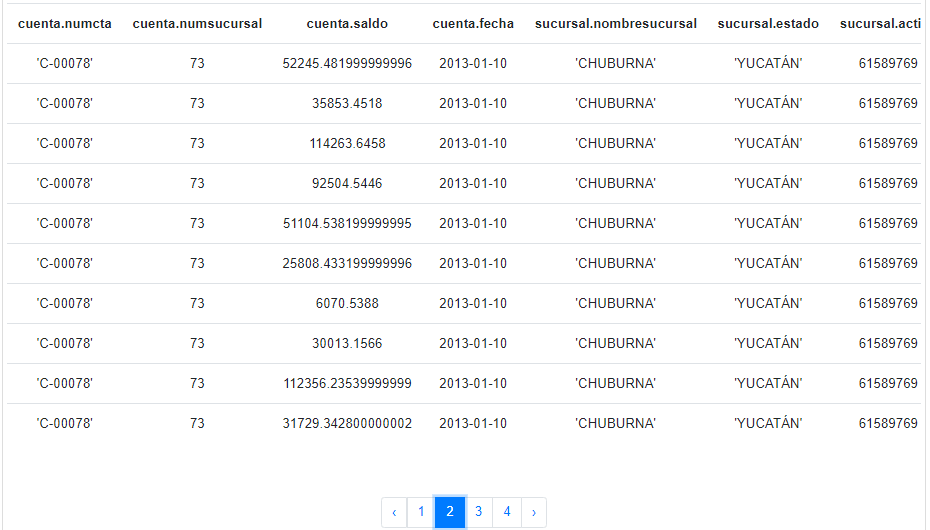
\includegraphics[scale=0.4]{psets/Tareas/Tarea03/Diagramas/2_2g3.png}
            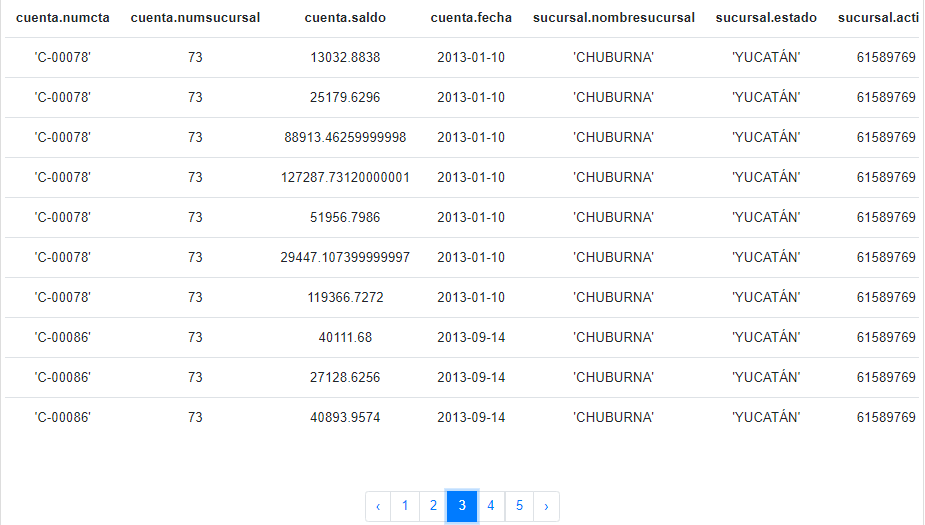
\includegraphics[scale=0.4]{psets/Tareas/Tarea03/Diagramas/2_2g4.png}   
            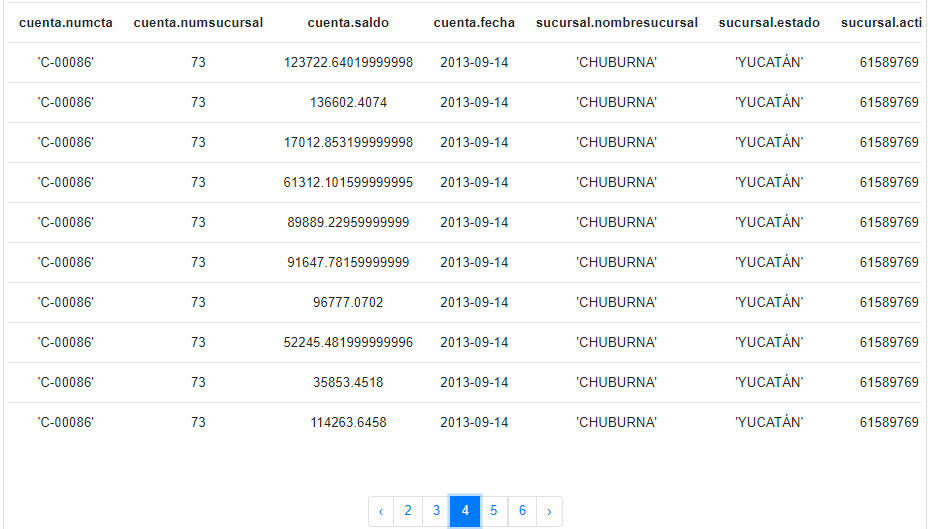
\includegraphics[scale=0.4]{psets/Tareas/Tarea03/Diagramas/2_2g5.png} 
            \\y muchas mas paginas, como se ve en el arbol hay 729 resultados
            %h%
            \item Aumentar \textbf{8}$\%$ a las cuentas con saldo mayor a $\$$\textbf{75,000} y a las demás en un 3$\%$. Las cuentas deben estar ubicadas en la sucursal \textbf{TEHUANTEPEC}.
            \begin{center}
            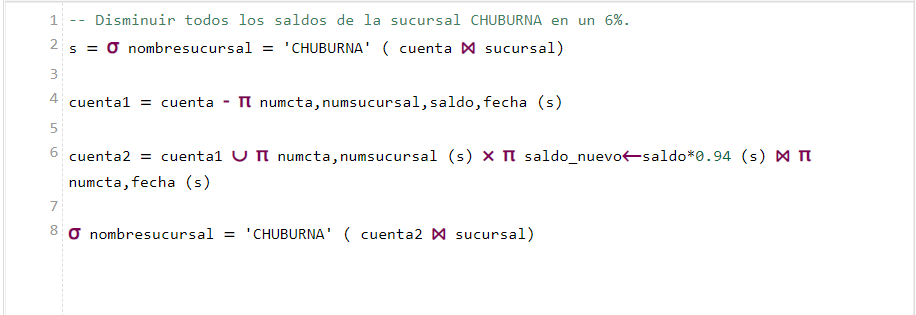
\includegraphics[scale=0.8]{psets/Tareas/Tarea03/Diagramas/2_2g0.png}
            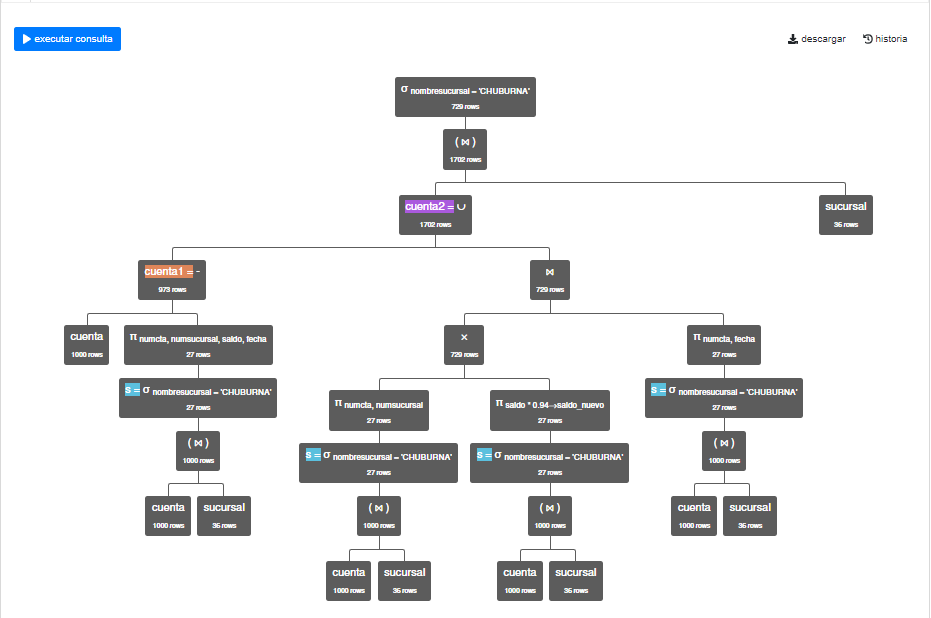
\includegraphics[scale=0.8]{psets/Tareas/Tarea03/Diagramas/2_2g1.png}
            \end{center}
            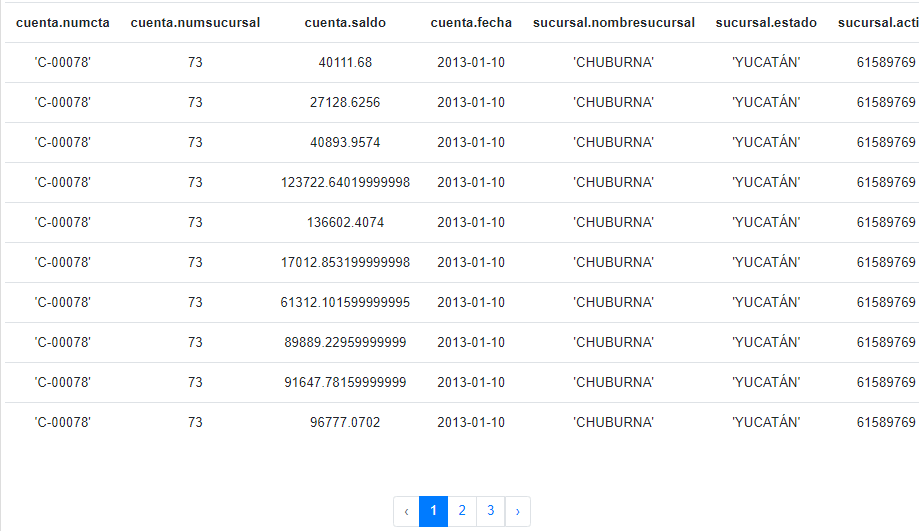
\includegraphics[scale=0.4]{psets/Tareas/Tarea03/Diagramas/2_2g2.png}    
            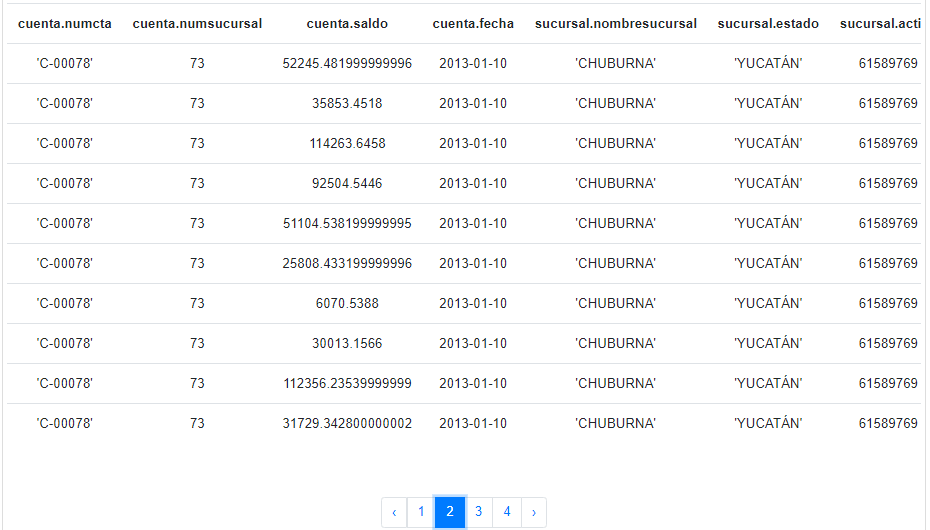
\includegraphics[scale=0.4]{psets/Tareas/Tarea03/Diagramas/2_2g3.png}
            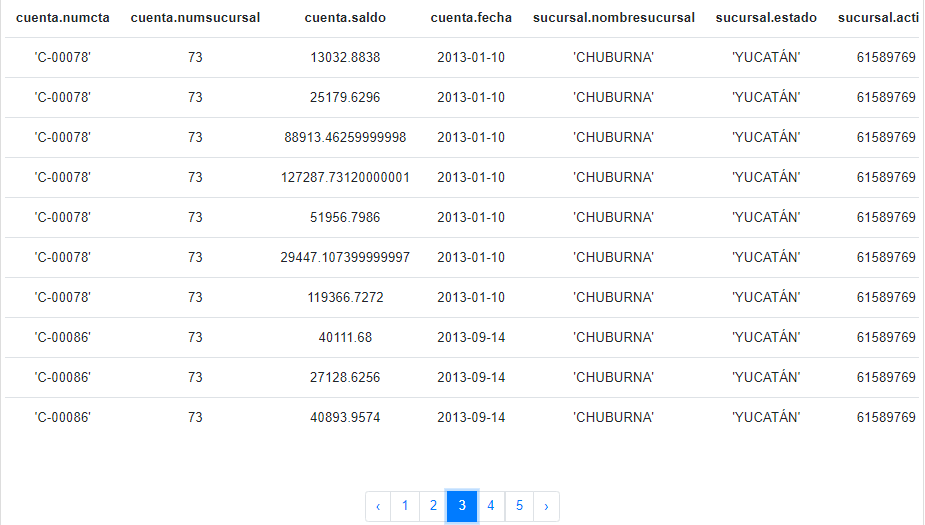
\includegraphics[scale=0.4]{psets/Tareas/Tarea03/Diagramas/2_2g4.png}   
            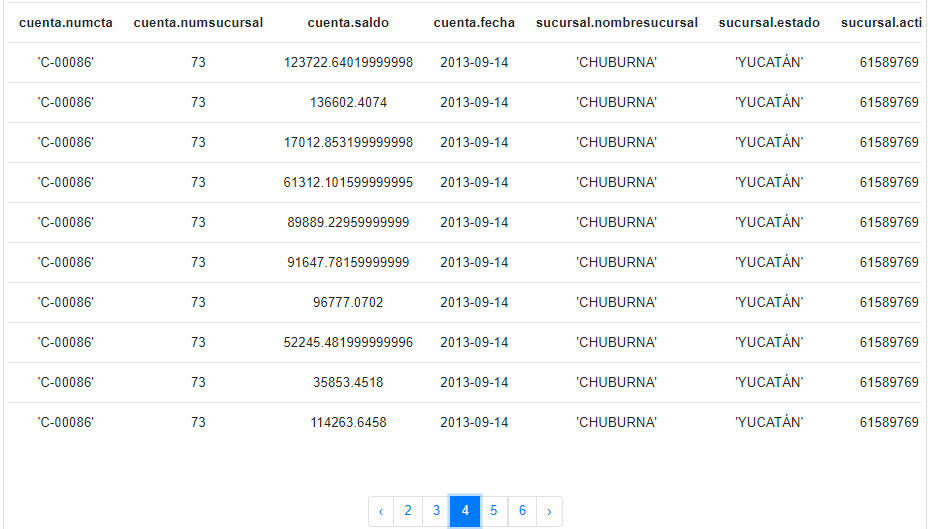
\includegraphics[scale=0.4]{psets/Tareas/Tarea03/Diagramas/2_2g5.png} 
            \\y muchas mas paginas, como se ve en el arbol hay 452 resultados
        \end{enumerate}
    \end{enumerate}
\end{document}